% main.tex
% ============================================================================
% A fresh, self-contained, geometric account of a method for embedding a
% multiset of n vectors in R^k injectively, continuously and permutation-
% invariantly, by a TWOFOLD barycentric subdivision followed by vertex hashing.
%
% Audience: a strong 1st/2nd-year Cambridge NatSci undergraduate.  Every term is
% defined; examples accompany each construction.  No reference to any code or
% prior write-up: this stands alone.
%
% The easy part (invariance, continuity) is dispatched quickly; the weight of
% the document is the INJECTIVITY argument and the explanation of why ONE
% subdivision does not suffice.
%
% Built incrementally.  Compile: pdflatex main; pdflatex main.
% ============================================================================

\documentclass[11pt,a4paper]{article}

\usepackage[margin=2.4cm]{geometry}
\usepackage{amsmath,amssymb}
\usepackage{amsthm}
\usepackage{enumitem}
\usepackage{xcolor}
\usepackage{tikz}
\usetikzlibrary{calc}
\usepackage[most]{tcolorbox}
\usepackage{hyperref}
\hypersetup{colorlinks=true,linkcolor=blue!55!black,urlcolor=blue!55!black}

% ── theorem-like environments ───────────────────────────────────────────────
\theoremstyle{definition}
\newtheorem{definition}{Definition}[section]
\newtheorem{example}[definition]{Example}
\newtheorem{remark}[definition]{Remark}
\theoremstyle{plain}
\newtheorem{theorem}[definition]{Theorem}
\newtheorem{proposition}[definition]{Proposition}
\newtheorem{lemma}[definition]{Lemma}
\newtheorem{corollary}[definition]{Corollary}

% ── a soft box for worked examples / intuition ──────────────────────────────
\tcbset{
  ideabox/.style={colback=blue!4,colframe=blue!40,boxrule=0.5pt,arc=2pt,
                  left=6pt,right=6pt,top=4pt,bottom=4pt},
}

% ── notation ─────────────────────────────────────────────────────────────────
\newcommand{\R}{\mathbb{R}}
\newcommand{\Sn}{S_n}
\newcommand{\bvec}[1]{\mathbf{#1}}
\newcommand{\bary}{\widehat}      % barycentre / canonical hat
\DeclareMathOperator{\sort}{sort}

\title{\bfseries Embedding multisets of vectors\\[2pt]
       \large A geometric method by twofold barycentric subdivision}
\author{}
\date{\today}

\begin{document}
\maketitle

\begin{abstract}
\noindent
We are given $n$ vectors in $\R^k$ with \emph{no preferred order} --- a
\emph{multiset} --- and we want to summarise them by a single point of some
$\R^N$ in a way that (i)~ignores the order, (ii)~loses no information, and
(iii)~varies continuously as the vectors move.  These three demands pull
against one another, and the naive fix (sorting) fails the third.  We describe a
method that meets all three.  Its engine is a classical piece of geometry ---
the \emph{barycentric subdivision} of a simplex --- applied \emph{twice}.
Order-invariance and continuity will be almost immediate.  The real work, and the
heart of this note, is the remaining demand, \emph{injectivity}: that distinct
multisets really do land on distinct points.  We give a geometric proof, and explain why a
\emph{single} subdivision is provably not enough.
\end{abstract}

\tableofcontents
\bigskip

% ════════════════════════════════════════════════════════════════════════════
\section{The problem}
\label{sec:problem}
% ════════════════════════════════════════════════════════════════════════════

\subsection{Multisets, and how we shall write them}

A \emph{multiset} is a collection in which repeats are allowed and counted, but
order is ignored.  Thus $\{3,3,5\}$ and $\{5,3,3\}$ are the \emph{same}
multiset, while $\{3,5\}$ and $\{3,3,5\}$ differ.  We are interested in
multisets of $n$ vectors drawn from $\R^k$.

We record such a multiset as a matrix.  Stack the $n$ vectors as the
\emph{columns} of a $k\times n$ matrix
\[
   M \;=\; \bigl[\ \bvec v_1\ \big|\ \bvec v_2\ \big|\ \cdots\ \big|\ \bvec v_n\ \bigr],
   \qquad \bvec v_j\in\R^k .
\]
Row $i$ of $M$ thus holds the $i$-th coordinate of every vector; column $j$
holds the whole of vector~$\bvec v_j$.  Because the vectors form a multiset, the
\emph{column order carries no meaning}: re-ordering the columns gives a
different matrix but the \emph{same} multiset.  Formally, the symmetric group
$\Sn$ (the group of all $n!$ permutations of $\{1,\dots,n\}$) acts on matrices
by permuting columns,
\[
   (\sigma\cdot M)\ \text{has $j$-th column}\ \bvec v_{\sigma^{-1}(j)},
   \qquad \sigma\in\Sn,
\]
and two matrices represent the same multiset exactly when one is obtained from
the other by such a column permutation. We write $M\sim M'$ in that case.

\begin{example}\label{ex:samemultiset}
With $n=3$, $k=2$,
\[
  M=\begin{bmatrix}4&1&4\\0&2&5\end{bmatrix}
  \quad\text{and}\quad
  M'=\begin{bmatrix}1&4&4\\2&5&0\end{bmatrix}
\]
represent the same multiset $\bigl\{\,(4,0),(1,2),(4,5)\,\bigr\}$: $M'$ is $M$
with its columns cyclically shifted.  Note that the two columns $(4,0)$ and
$(4,5)$ \emph{share their first entry} but are different vectors; multisets
happily contain such near-collisions, and our method must keep them apart.
\end{example}

\subsection{What we want to build}

We seek a map $f$ that sends a multiset $M$ (equivalently, its $\sim$-class) to a
point $f(M)\in\R^N$ for some fixed $N$, with three properties.

\begin{enumerate}[label=\textbf{(P\arabic*)},leftmargin=*]
\item \textbf{Permutation-invariance.} $f(M)=f(M')$ whenever $M\sim M'$. (The
      output depends only on the multiset, not on how we happened to list it.)
\item \textbf{Injectivity.} $f(M)=f(M')$ \emph{only} when $M\sim M'$. (Distinct
      multisets give distinct outputs --- no information is lost. A map that is
      both (P1) and (P2) is called an \emph{embedding}.)
\item \textbf{Continuity.} $f$ is continuous: nudging the vectors a little moves
      $f(M)$ only a little.
\end{enumerate}

\begin{remark}[why all three at once is awkward]\label{rmk:tension}
Any one or two of these is easy. The difficulty is all three together.
The obvious route to (P1) and (P2) is to \emph{sort}: agree on some fixed rule
for putting the columns in a canonical order (say, sort them
lexicographically), and read off the sorted matrix. Sorting certainly forgets
the original order (P1) and is reversible onto multisets (P2). But it is
\emph{not} continuous: as the vectors move and two of them swap places in the
sorted order, the canonical matrix jumps. Picture two columns of nearly equal
value sliding past each other --- at the instant they cross, the ``sort'' snaps
them into the opposite arrangement. So sorting buys (P1)+(P2) at the cost of
(P3). The art is to obtain the invariance of sorting \emph{without} its kinks.
\end{remark}

\begin{remark}[a harmless normalisation]\label{rmk:homog}
It is convenient, and costs nothing, to also ask for \emph{positive
homogeneity}: $f(\lambda M)=\lambda f(M)$ for scalars $\lambda>0$. Geometrically
this lets us think in terms of \emph{cones} and \emph{rays} rather than fussing
over overall scale, and the construction below provides it automatically. The
reader may ignore it on a first pass.
\end{remark}

\subsection{The plan, and where the difficulty lies}

The method has the following shape, and the rest of the document fills it in.
\begin{itemize}[leftmargin=*]
\item We first treat the easy case $k=1$ --- a multiset of $n$ \emph{numbers}
      --- because it already contains the central geometric idea in its
      simplest form (Section~\ref{sec:numbers}).
\item That idea is the \emph{barycentric subdivision} of a simplex, which we
      define from scratch and which turns the discontinuous ``sort'' into a
      continuous gadget.
\item For genuine vectors ($k\ge 2$) the rows interact, and we shall see that
      applying the idea once \emph{per row} is \emph{not enough} for injectivity
      --- a concrete pair of multisets collides. This failure, and its cure by a
      \emph{second} subdivision, is the crux (Sections~\ref{sec:rows}
      onward).
\item Finally a \emph{hashing} step turns the geometric data into a point of
      $\R^N$.
\end{itemize}

\noindent
Throughout, (P1) and (P3) will be easy to see as we go; the burden of proof is
(P2), injectivity, and in particular \emph{why two subdivisions are needed and
one is not}. That is the non-trivial content.

% ════════════════════════════════════════════════════════════════════════════
\section{The geometric idea: barycentric subdivision}
\label{sec:bary}
% ════════════════════════════════════════════════════════════════════════════

Before any multisets, we recall the one piece of geometry the whole method runs
on. It is elementary and classical; we set it up carefully because everything
later is an echo of it.

\subsection{The simplex and barycentric coordinates}

Fix $n$ points $\bvec e_1,\dots,\bvec e_n$ in general position (no three on a
line, etc.). Their \emph{simplex} is the solid region they span,
\[
   \Delta \;=\; \Bigl\{\ \textstyle\sum_{i=1}^n \alpha_i\,\bvec e_i\ :\
        \alpha_i\ge 0,\ \textstyle\sum_i\alpha_i=1\ \Bigr\}.
\]
For $n=3$ this is a (filled) triangle; for $n=4$ a tetrahedron. The numbers
$(\alpha_1,\dots,\alpha_n)$ are the \emph{barycentric coordinates} of the point
$\sum_i\alpha_i\bvec e_i$. The defining fact of a simplex is that
\emph{barycentric coordinates are unique}: each point of $\Delta$ is
$\sum_i\alpha_i\bvec e_i$ for exactly one choice of weights $\alpha_i\ge0$
summing to~$1$. A weight $\alpha_i$ is zero exactly when the point lies on the
face opposite $\bvec e_i$.

The \emph{barycentre} of a set of vertices is their average. The barycentre of
the whole simplex is $\bvec g=\tfrac1n(\bvec e_1+\dots+\bvec e_n)$ (all weights
equal); the barycentre of an edge $\bvec e_i\bvec e_j$ is its midpoint
$\tfrac12(\bvec e_i+\bvec e_j)$, and so on.

\subsection{Subdividing the simplex}

\emph{Barycentric subdivision} cuts $\Delta$ into smaller simplices using these
barycentres. The recipe, for our purposes, is cleanest stated through
\emph{orderings}. Given an ordering $\sigma$ of the vertices --- say
$\bvec e_{\sigma(1)},\bvec e_{\sigma(2)},\dots,\bvec e_{\sigma(n)}$ --- form the
running barycentres of its \emph{prefixes}:
\begin{equation}\label{eq:facebary}
   \bvec f^{\sigma}_r \;=\; \frac1r\bigl(\bvec e_{\sigma(1)}+\bvec e_{\sigma(2)}
            +\cdots+\bvec e_{\sigma(r)}\bigr),
   \qquad r=1,2,\dots,n .
\end{equation}
So $\bvec f^\sigma_1=\bvec e_{\sigma(1)}$ is a vertex, $\bvec f^\sigma_2$ is an
edge-midpoint, \dots, and $\bvec f^\sigma_n=\bvec g$ is the centre of the whole
simplex (the same point for every $\sigma$). These $n$ points span a small
simplex, the \emph{cell} $C_\sigma$. As $\sigma$ ranges over all $n!$ orderings,
the cells $C_\sigma$ tile $\Delta$ without overlap (Figure~\ref{fig:sd}).

\begin{figure}[h]
\centering
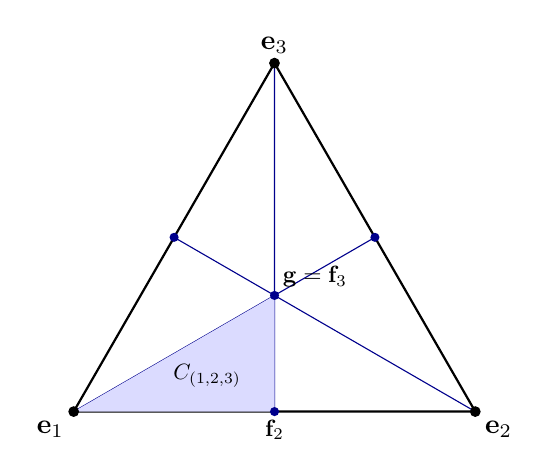
\begin{tikzpicture}[scale=1.5,line join=round]
  \coordinate (e1) at (0,0);
  \coordinate (e2) at (3.4,0);
  \coordinate (e3) at (1.7,2.95);
  \coordinate (m12) at ($(e1)!0.5!(e2)$);
  \coordinate (m13) at ($(e1)!0.5!(e3)$);
  \coordinate (m23) at ($(e2)!0.5!(e3)$);
  \coordinate (g)   at (barycentric cs:e1=1,e2=1,e3=1); % true centroid (2/3 down each median)
  % outer triangle
  \draw[thick] (e1)--(e2)--(e3)--cycle;
  % medians (the subdivision)
  \draw[blue!55!black] (e1)--(m23);
  \draw[blue!55!black] (e2)--(m13);
  \draw[blue!55!black] (e3)--(m12);
  % one cell shaded: order (1,2,3): e1 -> m12 -> g
  \fill[blue!14] (e1)--(m12)--(g)--cycle;
  % vertices and barycentres
  \foreach \p/\pos/\lab in {e1/below left/{$\bvec e_1$}, e2/below right/{$\bvec e_2$},
        e3/above/{$\bvec e_3$}}{\fill (\p) circle (1.3pt); \node[\pos] at (\p) {\lab};}
  \foreach \p/\pos/\lab in {m12/below/{$\bvec f_2$}, m13/left/{}, m23/right/{},
        g/above right/{$\bvec g=\bvec f_3$}}{\fill[blue!55!black] (\p) circle (1.1pt); \node[\pos,scale=0.85] at (\p) {\lab};}
  \node[scale=0.8] at (1.13,0.30) {$C_{(1,2,3)}$}; % centre of the (corrected) 1/6 cell e1-f2-g
\end{tikzpicture}
\caption{Barycentric subdivision of a triangle ($n=3$): the three medians cut it
into $3!=6$ cells, one per ordering of the vertices. The shaded cell
$C_{(1,2,3)}$ has vertices $\bvec f_1=\bvec e_1$, $\bvec f_2=\tfrac12(\bvec
e_1{+}\bvec e_2)$ and $\bvec f_3=\bvec g=\tfrac13(\bvec e_1{+}\bvec e_2{+}\bvec
e_3)$. The centre $\bvec g$ is shared by all six cells.}
\label{fig:sd}
\end{figure}

\subsection{The one fact we shall use again and again}

Here is the property that makes the subdivision useful. It says that locating a
point among the cells is a \emph{continuous} substitute for sorting.

\begin{proposition}[unique cell, unique coordinates]\label{prop:cell}
Let $p=\sum_i\alpha_i\bvec e_i$ be a point of $\Delta$, and let $\sigma$ be an
ordering that sorts its weights into non-increasing order,
$\alpha_{\sigma(1)}\ge\alpha_{\sigma(2)}\ge\cdots\ge\alpha_{\sigma(n)}$. Then $p$
lies in the cell $C_\sigma$, and its barycentric coordinates there are, up to the
factor $r$, the \emph{gaps} $\alpha_{\sigma(r)}-\alpha_{\sigma(r+1)}$ between
consecutive sorted weights:
\begin{equation}\label{eq:gaps}
   \beta_r \;=\; r\,\bigl(\alpha_{\sigma(r)}-\alpha_{\sigma(r+1)}\bigr)\ \ge 0,
   \qquad (\alpha_{\sigma(n+1)}:=0),
\end{equation}
so that $p=\sum_{r=1}^n \beta_r\,\bvec f^\sigma_r$ with $\beta_r\ge0$ and
$\sum_r\beta_r=1$. If the sorting order is \emph{strict} the cell is unique; if
two weights are tied, $\alpha_{\sigma(r)}=\alpha_{\sigma(r+1)}$, then the
corresponding gap, and so $\beta_r$, is \emph{zero}, and $p$ lies on a wall
shared by the two cells that differ only by swapping those two ranks.
\end{proposition}

\begin{proof}[Why this is true]
That \eqref{eq:gaps} reproduces $p$ is the discrete ``summation by parts''
identity $\sum_i\alpha_i\bvec e_i=\sum_r r(\alpha_{\sigma(r)}-\alpha_{\sigma(r+1)})
\bvec f^\sigma_r$, which one checks by expanding $\bvec f^\sigma_r$ from
\eqref{eq:facebary} and collecting the coefficient of each $\bvec e_{\sigma(r)}$
(it telescopes back to $\alpha_{\sigma(r)}$). The gaps are $\ge0$ precisely
because the weights were sorted, which is what places $p$ in $C_\sigma$; and a
tie makes a gap vanish, putting $p$ on the boundary face where that barycentre
drops out. Uniqueness of the $\beta_r$ is uniqueness of barycentric coordinates
in the cell.
\end{proof}

\begin{tcolorbox}[ideabox]
\textbf{The point of Proposition~\ref{prop:cell}.} ``Which cell?'' is decided by
the \emph{order} of the weights --- a discrete, sorting-like datum. But the
\emph{coordinates} $\beta_r$ vary continuously, and exactly when the order is
ambiguous (a tie) the ambiguous coordinate is $0$, so the point sits cleanly on
a shared wall and nothing jumps. This is how a subdivision launders the
discontinuity out of sorting: \emph{the place where the cell-label is ambiguous
is exactly the place where it does not matter.}
\end{tcolorbox}

% ════════════════════════════════════════════════════════════════════════════
\section{Warm-up: a multiset of numbers ($k=1$)}
\label{sec:numbers}
% ════════════════════════════════════════════════════════════════════════════

Take the simplest case first: $k=1$, so each ``vector'' is a single number and
the data is a multiset of $n$ reals $x_1,\dots,x_n$, written as the single row
$M=[\,x_1\ \cdots\ x_n\,]$. This already contains the heart of the idea, and
solving it cleanly tells us precisely what will be \emph{missing} when $k\ge2$.

\subsection{The same picture, in a cone}

Proposition~\ref{prop:cell} was about a simplex (weights summing to $1$). The
identical statement holds, even more simply, in the positive ``orthant''
$\{\,x\in\R^n:x_i\ge0\,\}$ if we drop the sum-to-one condition. Sort the entries
of $x$ into non-increasing order, $x_{(1)}\ge x_{(2)}\ge\cdots\ge x_{(n)}\ge0$,
and form the \emph{prefix vectors}
\[
   \bvec u_r \;=\; \bvec e_{(1)}+\bvec e_{(2)}+\cdots+\bvec e_{(r)}
   \qquad(\text{the indicator of the top-$r$ positions}),
\]
where $\bvec e_{(s)}$ is the standard basis vector for the position holding the
$s$-th largest entry. Then summation by parts gives, just as in
\eqref{eq:gaps},
\begin{equation}\label{eq:numdecomp}
   x \;=\; \sum_{r=1}^{n}\ \delta_r\,\bvec u_r,
   \qquad
   \delta_r=x_{(r)}-x_{(r+1)}\ \ge 0,\quad (x_{(n+1)}:=0).
\end{equation}
The coefficients $\delta_r$ are the \emph{gaps} between consecutive sorted
values; $\delta_n=x_{(n)}$ is the smallest entry, attached to the all-ones
vector $\bvec u_n=\bvec e_1+\cdots+\bvec e_n$. (Geometrically the $\bvec u_r$ are
just the face-barycentres $\bvec f_r$ of \eqref{eq:facebary} un-normalised by the
factor $1/r$; nothing has changed but the bookkeeping of scale.)

\begin{example}\label{ex:numbers}
For $x=(2,9,2,6)$, sorting gives $9\ge6\ge2\ge2$, so the gaps are
$\delta_1=9{-}6=3$, $\delta_2=6{-}2=4$, $\delta_3=2{-}2=0$, $\delta_4=2$. The
prefixes are: top-$1=\{$the $9\}$, top-$2=\{9,6\}$, top-$3=\{9,6,2\}$,
top-$4=$ everything. The vanishing gap $\delta_3=0$ records the tie between the
two $2$'s --- and note it makes the (ambiguous: \emph{which} $2$?) top-$3$
prefix irrelevant, since it is multiplied by $0$.
\end{example}

\subsection{Reading off the invariant, and why all three properties hold}

To turn \eqref{eq:numdecomp} into something that forgets the labelling, observe
what survives relabelling. Permuting the $n$ numbers permutes the standard basis
vectors, hence relabels \emph{which} positions sit in each prefix --- but it
changes neither the gaps $\delta_r$ nor the \emph{sizes} of the prefixes. And
for a multiset of bare numbers, a prefix carries no information beyond its
size: any two top-$r$ sets are interchangeable. So the honest, label-free record
of $x$ is simply the list of pairs
\[
   \bigl\{\,(\delta_r,\ r)\ :\ r=1,\dots,n\,\bigr\}
   \qquad\text{(gap, prefix-size)},
\]
which is no more and no less than the sorted gaps. Let this be $f(M)$ (we shall
hash it into a single $\R^N$ point later; for now its content is what matters).

\begin{itemize}[leftmargin=*]
\item \textbf{(P1) Invariance} is immediate: gaps and sizes do not depend on how
      the numbers were listed.
\item \textbf{(P2) Injectivity} holds because the data is reversible: from the
      gaps we rebuild the sorted values ($x_{(r)}=\delta_r+\delta_{r+1}+\cdots
      +\delta_n$), and the sorted values \emph{are} the multiset.
\item \textbf{(P3) Continuity} holds because each gap $\delta_r$ is a continuous
      function of the multiset (order statistics move continuously), the sizes
      $r$ are fixed integers, and --- crucially --- at any tie the moving gap is
      $0$, so no quantity jumps. This is exactly the laundering of
      Proposition~\ref{prop:cell}: we never had to commit to \emph{which}
      tied number was ``larger''.
\end{itemize}

\noindent
So for $k=1$ a \emph{single} barycentric subdivision already does everything.

\subsection{The crack that opens at $k\ge2$}
\label{sec:crack}

Look hard at why injectivity was so cheap above: a prefix mattered only through
its \emph{size}, so ``canonicalising'' it (forgetting the labels) lost nothing
we needed. That is special to one row.

With $k\ge2$ rows, the columns are shared: a single permutation reorders the
columns of \emph{every} row at once. Now a prefix in row $i$ is a genuine
\emph{subset of the $n$ columns}, and --- because the same columns recur in
every row --- \emph{which} columns it contains, not merely how many, can matter.
Two multisets can agree row-by-row on all the gaps and all the prefix-sizes, yet
differ in how the prefixes of \emph{different rows line up over the shared
columns}. Forgetting the column labels one row at a time would erase exactly
that cross-row alignment.

Section~\ref{sec:rows} makes this precise and exhibits two genuinely different
multisets that a one-subdivision-per-row scheme cannot tell apart. Repairing
the damage is what the \emph{second} subdivision is for.

% ════════════════════════════════════════════════════════════════════════════
\section{Vectors, and why one subdivision is not enough}
\label{sec:rows}
% ════════════════════════════════════════════════════════════════════════════

Now let $k\ge2$. We apply the warm-up idea to \emph{each row} of $M$ and watch it
fall short.

\subsection{The first subdivision, applied row by row}

Each row of $M$ is a list of $n$ numbers, so Section~\ref{sec:numbers} applies to
it verbatim. Sorting row $i$ and decomposing as in \eqref{eq:numdecomp} writes
that row as a sum of gaps times prefixes. The novelty is purely in the
bookkeeping of \emph{which columns} a prefix contains, so we name these objects
once and for all --- they are the raw material of everything that follows.

\begin{definition}[piece]\label{def:piece}
Fix a row $i$ and a level $r\in\{1,\dots,n-1\}$. Sorting row $i$ singles out its
\emph{top-$r$ prefix}: the set of the $r$ columns carrying that row's largest $r$
entries. The associated \emph{piece} is the $k\times n$ matrix $P$ that holds the
$0/1$ indicator of this prefix in row $i$ and is zero in every other row. We say
$P$ \emph{sits in row $i$} and has \emph{size $r$}, and we attach to it the
\emph{gap} $\delta^{(i)}_r\ge0$ of \eqref{eq:numdecomp}. There are exactly
$m=k(n-1)$ pieces --- $(n-1)$ per row --- and, because the prefixes within a row
are nested, a piece is pinned down by its $(\textit{row},\textit{size})$ alone.
\end{definition}

\noindent
A piece is thus one rung of a single row's prefix ladder, lifted into a
$k\times n$ matrix so that pieces from \emph{different} rows inhabit a common
space and can be added. From here on, pieces (and sums of them) are the only
objects we manipulate.

\begin{example}\label{ex:firstsd}
Let $n=2$, $k=2$ and
\[
   A=\begin{bmatrix}3&0\\[1pt]0&2\end{bmatrix}.
\]
Row $1=(3,0)$: top-$1$ prefix is column~$1$, gap $\delta^{(1)}_1=3$. Row
$2=(0,2)$: top-$1$ prefix is column~$2$, gap $\delta^{(2)}_1=2$. As pieces (the
all-ones size-$2$ prefixes carry the row minima, here $0$, so we drop them):
\[
  \underbrace{\begin{bmatrix}1&0\\0&0\end{bmatrix}}_{\text{row-1 top, gap }3}
  \qquad
  \underbrace{\begin{bmatrix}0&0\\0&1\end{bmatrix}}_{\text{row-2 top, gap }2}.
\]
The whole of $A$ (above its row minima) is $3\cdot\text{(first piece)}+2\cdot
\text{(second piece)}$.
\end{example}

So after the first subdivision the data is: for each row, a sorted list of
\emph{(gap, prefix)} pairs, the prefixes being subsets of the $n$ shared
columns.

\subsection{The naive repair, and what it really quotients by}

To make this permutation-invariant we must forget the column labels. The
warm-up did so by keeping only prefix \emph{sizes}. If we do the same here ---
canonicalise each row's prefixes \emph{on their own}, recording each only up to
relabelling its columns --- we are quotienting each row \emph{separately} by its
own copy of $\Sn$. That is the product group $\Sn\times\cdots\times\Sn$ ($k$
copies), allowing a \emph{different} column permutation in every row.

But the symmetry we are actually entitled to is far smaller: a multiset permits
\emph{one} permutation applied to \emph{all} rows simultaneously --- the
\emph{diagonal} copy of $\Sn$ inside the product. Quotienting by the whole
product is coarser; it glues together matrices that are \emph{not} column
rearrangements of one another. We have thrown away the cross-row alignment
warned of in Section~\ref{sec:crack}. The next example shows this is fatal.

\subsection{Two multisets the naive scheme cannot separate}

\begin{example}[the collision]\label{ex:collision}
Keep $n=2$, $k=2$ and set, alongside $A$ above,
\[
   A=\begin{bmatrix}3&0\\0&2\end{bmatrix},
   \qquad
   B=\begin{bmatrix}3&0\\2&0\end{bmatrix}.
\]
These are \emph{different multisets}:
\[
   A=\bigl\{\,(3,0),\,(0,2)\,\bigr\},
   \qquad
   B=\bigl\{\,(3,2),\,(0,0)\,\bigr\},
\]
and no reordering of two columns turns one into the other ($A$ has two vectors
each with a single zero entry; $B$ has the vector $(3,2)$ and the zero vector).

Yet run the naive per-row scheme. In \emph{both} matrices:
\begin{itemize}[nosep,leftmargin=*]
\item row~$1$ is $(3,0)$ --- gap $3$, one top prefix of size $1$, row-min $0$;
\item row~$2$ is $(2,0)$ or $(0,2)$ --- either way gap $2$, one top prefix of
      size $1$, row-min $0$.
\end{itemize}
Row by row, after forgetting which column is which, the recorded data is
identical: \{row 1: gap $3$, size $1$\}, \{row 2: gap $2$, size $1$\}. The naive
scheme returns the \emph{same} answer for $A$ and $B$. It is \textbf{not
injective}. The single fact it could not see is whether the two rows' top
columns are the \emph{same} column (as in $B$) or \emph{different} columns
(as in $A$) --- precisely a statement about how the rows align over the shared
labels, which no amount of per-row canonicalisation can recover.
\end{example}

\subsection{The cure, in one sentence}

The defect is that we canonicalised \emph{row-local} objects. To respect only
the diagonal $\Sn$, we must canonicalise objects that \emph{span all the rows at
once}, so that a single column permutation acts on all of them together. The
cheapest such objects are \emph{sums of pieces drawn from different rows}: a
single $k\times n$ matrix in which several rows are simultaneously populated.

Watch how this already rescues Example~\ref{ex:collision}. Add the two pieces
of each matrix into one cross-row matrix:
\[
   A:\ \begin{bmatrix}1&0\\0&0\end{bmatrix}+\begin{bmatrix}0&0\\0&1\end{bmatrix}
      =\begin{bmatrix}1&0\\0&1\end{bmatrix},
   \qquad
   B:\ \begin{bmatrix}1&0\\0&0\end{bmatrix}+\begin{bmatrix}0&0\\1&0\end{bmatrix}
      =\begin{bmatrix}1&0\\1&0\end{bmatrix}.
\]
Now canonicalise by sorting the \emph{columns} of each (one permutation for the
whole matrix). The columns of $A$'s matrix are $(1,0)$ and $(0,1)$; of $B$'s,
$(1,1)$ and $(0,0)$. These are different as multisets of columns, so the
canonical forms \emph{differ}: the cross-row sum sees what the per-row data
could not --- namely whether the two top entries share a column. A single matrix
can only be tidied by a single column permutation, which is exactly the diagonal
symmetry we are allowed.

\medskip\noindent
This is the whole reason for a \emph{second} subdivision: it is the systematic,
continuous way to manufacture and weight these cross-row matrices. We turn to it
next.

% ════════════════════════════════════════════════════════════════════════════
\section{The second subdivision, and the finished method}
\label{sec:second}
% ════════════════════════════════════════════════════════════════════════════

\subsection{Pooling the pieces}

After the first subdivision (one per row) we hold a bag of $m=k(n-1)$
\emph{(gap, piece)} pairs --- $(n-1)$ proper prefixes from each of the $k$ rows.
(The $k$ all-ones, size-$n$ prefixes are fully symmetric: a column permutation
fixes each of them. They carry no alignment information, so we set them aside as
$k$ \emph{anchors}, namely the $k$ row minima $m_1,\dots,m_k$, which are
plainly permutation-invariant numbers; we record them directly and forget them
for now.)

Crucially, this bag is \emph{itself} a point in a cone --- the cone spanned by
the $m$ pieces, with the gaps as coordinates:
\[
   (\text{balance of }M)\;=\;\sum_{\text{pieces }P}\ \delta_P\, P .
\]
So we may apply the \emph{very same} barycentric subdivision a second time, now
to this $m$-piece cone, with the pieces playing the role the standard basis
vectors $\bvec e_i$ played before.

\subsection{The second subdivision}

Sort the $m$ pieces into non-increasing gap order, $\delta_{(1)}\ge\delta_{(2)}
\ge\cdots\ge\delta_{(m)}$, and (Proposition~\ref{prop:cell}, in the cone form
\eqref{eq:numdecomp}, applied to the pieces) form the running sums
\begin{equation}\label{eq:Ls}
   L_s \;=\; P_{(1)}+P_{(2)}+\cdots+P_{(s)},
   \qquad
   \alpha_s \;=\; \delta_{(s)}-\delta_{(s+1)}\ \ge0,
\end{equation}
for $s=1,\dots,m$ (with $\delta_{(m+1)}:=0$), so that, by summation by parts,
$\text{balance}=\sum_t\delta_{(t)}P_{(t)}=\sum_s\alpha_s L_s$. Each $L_s$ is a single $k\times n$
matrix of non-negative integers --- a \emph{cross-row} object, exactly the kind
Section~\ref{sec:rows} said we needed: it is the running total of the
highest-gap pieces, and because those pieces come from \emph{different rows} it
populates several rows at once. We call $L_s$ a \emph{cumulative matrix}.

\begin{remark}
This is genuinely the same operation as the first subdivision --- ``sort, then
take running barycentres'' --- but now the things being sorted are whole pieces,
not numbers within a row, and the running sums knit the rows together. The two
applications differ only in what they are applied to: \emph{within each row}
first, then \emph{across the pooled pieces}.
\end{remark}

\begin{example}[the second subdivision, worked]\label{ex:secondsd}
Take $n=3$, $k=2$ and
\[
   M=\begin{bmatrix}6&1&2\\4&10&1\end{bmatrix}.
\]
Both row minima equal $1$, so the anchors are $m_1=m_2=1$; subtracting them
leaves the balance $\left[\begin{smallmatrix}5&0&1\\3&9&0\end{smallmatrix}\right]$.
The first subdivision (Definition~\ref{def:piece}) produces four pieces, shown
here with their gaps:
\[
 \underbrace{\left[\begin{smallmatrix}1&0&0\\0&0&0\end{smallmatrix}\right]}
   _{\text{row 1, size 1; gap }4}\qquad
 \underbrace{\left[\begin{smallmatrix}1&0&1\\0&0&0\end{smallmatrix}\right]}
   _{\text{row 1, size 2; gap }1}\qquad
 \underbrace{\left[\begin{smallmatrix}0&0&0\\0&1&0\end{smallmatrix}\right]}
   _{\text{row 2, size 1; gap }6}\qquad
 \underbrace{\left[\begin{smallmatrix}0&0&0\\1&1&0\end{smallmatrix}\right]}
   _{\text{row 2, size 2; gap }3}
\]
Pooling and sorting by gap ($6\ge4\ge3\ge1$) orders the pieces as
$P_{(1)},\dots,P_{(4)}$, and the running sums \eqref{eq:Ls} are the cumulative
matrices
\[
 \underbrace{\left[\begin{smallmatrix}0&0&0\\0&1&0\end{smallmatrix}\right]}
   _{L_1,\ \alpha_1=2}\qquad
 \underbrace{\left[\begin{smallmatrix}1&0&0\\0&1&0\end{smallmatrix}\right]}
   _{L_2,\ \alpha_2=1}\qquad
 \underbrace{\left[\begin{smallmatrix}1&0&0\\1&2&0\end{smallmatrix}\right]}
   _{L_3,\ \alpha_3=2}\qquad
 \underbrace{\left[\begin{smallmatrix}2&0&1\\1&2&0\end{smallmatrix}\right]}
   _{L_4,\ \alpha_4=1}
\]
with weights $\alpha_s=\delta_{(s)}-\delta_{(s+1)}$ read off
$\delta=(6,4,3,1)$. As a check, $\sum_s\alpha_s L_s$ rebuilds the balance ---
e.g.\ its $(2,2)$ entry is $2{\cdot}1+1{\cdot}1+2{\cdot}2+1{\cdot}2=9$. Two
features to note for later: $L_s$ grows by exactly one piece at each step, and
the richest matrix $L_4$ has carried integer counts up to~$2$ --- the
``staircase'' that Section~\ref{sec:inj} will read back to recover everything.
\end{example}

\subsection{Canonicalise, and assemble the output}

Finally make the result blind to the column labelling. Canonicalise each
cumulative matrix $L_s$ by sorting its columns into a fixed standard order
(say lexicographically); call the result $\bary L_s$. Because a single
permutation is applied to the whole matrix, this respects exactly the diagonal
$\Sn$. The output of the method is the collection
\begin{equation}\label{eq:output}
   f(M)\;=\;\Bigl(\ \underbrace{m_1,\dots,m_k}_{\text{anchors}}\ ;\
       \bigl\{\,(\bary L_s,\ \alpha_s)\ :\ \alpha_s>0\,\bigr\}\ \Bigr).
\end{equation}
(Pairs with $\alpha_s=0$ contribute nothing and are dropped.) A final
\emph{hashing} step, Section~\ref{sec:hash}, compresses this into a single point
of $\R^N$; but \eqref{eq:output} already holds all the information, so we argue
about it directly.

\subsection{Invariance, continuity and homogeneity are immediate}

As promised, the easy properties cost almost nothing.

\begin{proposition}[(P1), (P3) and homogeneity]\label{prop:easy}
The map \eqref{eq:output} is permutation-invariant, continuous, and positively
homogeneous of degree~$1$: $f(\lambda M)=\lambda f(M)$ for every $\lambda>0$.
The last point settles Remark~\ref{rmk:homog}.
\end{proposition}

\begin{proof}
\emph{(P1)} A column permutation $\sigma$ relabels the columns of every row
identically, hence permutes the columns of every piece, hence of every
cumulative matrix $L_s$, by the same $\sigma$; sorting the columns
($L_s\mapsto\bary L_s$) erases it. The gaps, and therefore the weights
$\alpha_s$ and the anchors $m_i$, are computed from sorted values and are
unchanged by $\sigma$. So $f(\sigma\cdot M)=f(M)$.

\emph{(P3)} Both subdivisions are instances of
Proposition~\ref{prop:cell}, whose coordinates (gaps, then the $\alpha_s$) are
continuous, with the saving grace that whenever an ordering is ambiguous --- two
tied row-values, or two tied gaps --- the corresponding coordinate is $0$. A
cumulative matrix $L_s$ whose existence depends on breaking such a tie is
therefore weighted by $\alpha_s=0$ and is dropped, so the (discontinuous) choice
of how to break the tie never reaches the output. Hence $f$ is continuous. (The
anchors $m_i$ are continuous as minima.)

\emph{Homogeneity.} Scaling $M\mapsto\lambda M$ with $\lambda>0$ multiplies every
entry, hence every row minimum ($m_i\mapsto\lambda m_i$) and every gap
($\delta\mapsto\lambda\delta$, so $\alpha_s\mapsto\lambda\alpha_s$), by
$\lambda$ --- but it changes no \emph{order}. So the sort orders, the pieces, and
the cumulative matrices $L_s$, being purely combinatorial, are untouched; each
$\bary L_s$ is identical, while every coordinate $\alpha_s$ and anchor $m_i$
scales by $\lambda$. Thus the whole output \eqref{eq:output}, and its hash
\eqref{eq:hash}, scales by $\lambda$. This is exactly why it paid to work
throughout with \emph{cones and rays} rather than normalising: the combinatorial
skeleton (which cells, which pieces) is scale-free, and only the coordinates
carry the scale.
\end{proof}

\noindent
That disposes of (P1) and (P3). Everything now turns on (P2).

% ════════════════════════════════════════════════════════════════════════════
\section{Injectivity}
\label{sec:inj}
% ════════════════════════════════════════════════════════════════════════════

This is the substance of the note. We show that the output \eqref{eq:output}
determines the multiset. Two simple observations do all the work; the second
subdivision earns its keep in both.

\subsection{A cumulative matrix remembers its pieces}

The pieces summed into a cumulative matrix are not lost in the sum --- they can
be read straight back off. The reason is that the pieces from a given row are
\emph{nested}: in row $i$ the contributing prefixes are some of
$\text{top-}1\subset\text{top-}2\subset\cdots$, so the count in column $c$ simply
records how many of them reach that column.

\begin{lemma}[recovery]\label{lem:recover}
From a cumulative matrix $L$ one can recover exactly which pieces were summed to
build it. Concretely, in each row $i$ the sets of columns
\[
   \{\,c:\ L_{i,c}\ge t\,\},\qquad t=1,2,3,\dots
\]
are precisely the contributing prefixes of row $i$, listed from largest~$t$
(smallest prefix) upward.
\end{lemma}

\begin{proof}
Row $i$ of $L$ is a sum of indicators of nested prefixes
$Q_1\subset Q_2\subset\cdots\subset Q_a$ (those present in row $i$). The entry in
column $c$ counts how many $Q_b$ contain $c$. Because the $Q_b$ are nested, the
columns with entry $\ge t$ are exactly those lying in the $t$-th largest of them,
i.e.\ in $Q_{a-t+1}$. So thresholding at $t=1,2,\dots$ returns
$Q_a,Q_{a-1},\dots,Q_1$ --- all the contributing prefixes, columns and all.
\end{proof}

\begin{example}\label{ex:staircase}
Suppose a row of some $L$ reads $(2,0,3,1)$. Columns with entry $\ge1$ are
$\{1,3,4\}$; with entry $\ge2$, $\{1,3\}$; with entry $\ge3$, $\{3\}$; nothing
reaches $4$. So this row was built from the three nested prefixes
$\{3\}\subset\{1,3\}\subset\{1,3,4\}$ --- the top-$1$, top-$2$ and top-$3$ sets
of that row --- and we have recovered them, columns included, from the row
alone.
\end{example}

Two consequences will be used repeatedly.

\begin{corollary}[pieces are named by (row, size)]\label{cor:rowsize}
Within any row the contributing prefixes are nested, so there is \emph{at most
one} of each size. Hence every piece is unambiguously named by the pair
$(\text{row},\ \text{size})$, and this name is permutation-invariant (column
sorting changes neither a piece's row nor its size).
\end{corollary}

\begin{corollary}[recovery survives canonicalisation]\label{cor:survive}
Sorting the columns of $L$ permutes all rows by one permutation $\sigma$, which
turns each recovered prefix $Q$ into $\sigma(Q)$ but leaves its \emph{size}, and
the \emph{nesting}, untouched. So from the canonical $\bary L$ we still recover
the piece-set --- as a set of $(\text{row},\text{size})$ names, exactly --- and
the actual columns up to the single permutation $\sigma$.
\end{corollary}

\subsection{The injectivity theorem}

\begin{theorem}\label{thm:inj}
The map $f$ of \eqref{eq:output} is injective on multisets: if $f(M)=f(M')$ then
$M\sim M'$.
\end{theorem}

The proof separates cleanly into a \emph{combinatorial} part that needs no
column labels at all, and a single \emph{alignment} step that fixes the labels
once, using one matrix.

\begin{proof}
Suppose we are handed the output \eqref{eq:output}: the anchors $m_1,\dots,m_k$
and the multiset of pairs $\{(\bary L_s,\alpha_s):\alpha_s>0\}$. We reconstruct
$M$ up to a column permutation.

\smallskip
\emph{Step 1 (combinatorics, no labels needed).}
By Lemma~\ref{lem:recover} and Corollary~\ref{cor:rowsize}, each $\bary L_s$
reveals its piece-set as a set of $(\text{row},\text{size})$ names --- and these
names are permutation-invariant, so there is \emph{no ambiguity} here. The
number of names is the size of the piece-set, which identifies the index $s$
(recall $L_s$ pooled the $s$ highest-gap pieces). Ordering the survivors by this
size gives a nested chain of piece-sets
\[
   \{P_{(1)}\}\subset\{P_{(1)},P_{(2)}\}\subset\cdots,
\]
each step naming the next piece in \emph{gap order} --- or, where several gaps
coincide, the next \emph{block} of equal-gap pieces, whose internal order is
immaterial. Thus the gap-ordering of the pieces is recovered (up to that
immaterial shuffling within tied blocks), as $(\text{row},\text{size})$ names. Moreover the
gaps themselves come back: since $\alpha_s=\delta_{(s)}-\delta_{(s+1)}$ we have
$\delta_{(s)}=\sum_{t\ge s}\alpha_t$, so each piece's gap is known. With the
anchors $m_i$, the sorted values of every row are now determined --- as numbers
attached to $(\text{row},\text{size})$ slots, still with no column labels in
sight.

\smallskip
\emph{Step 2 (one alignment, from one matrix).}
It remains to place the columns. Let $L^\ast$ be the \emph{richest} surviving
cumulative matrix --- the one whose piece-set is largest; it contains every
piece that occurs (a piece with positive gap appears in $L^\ast$, one with zero
gap is genuinely absent from $M$). By Corollary~\ref{cor:survive}, choosing any
column labelling that realises the canonical form $\bary L^\ast$ fixes a single
permutation $\sigma$, and in this labelling $L^\ast$ exhibits, in each row, the
\emph{whole} nested chain of that row's prefixes --- that is, which column is the
row's largest, second largest, and so on. One matrix thus pins the joint column
ranking of \emph{all} rows simultaneously, because all rows live in it together.

\smallskip
\emph{Assembly.}
Combine the two steps in the labelling $\sigma$: Step~1 supplies the value at
each (row, rank) slot; Step~2 supplies which column occupies each rank in each
row. Filling the values into the columns reconstructs the balance, and with the
anchors, the matrix $M$ --- uniquely up to the one permutation $\sigma$, i.e.\
up to $\sim$. Hence the output determines $M$ as a multiset, which is exactly
injectivity. (Where a gap is zero the two tied columns are interchangeable, so
the ambiguity is precisely a $\sim$-ambiguity and harms nothing.)
\end{proof}

\begin{tcolorbox}[ideabox]
\textbf{What made it work.} The combinatorics of Step~1 never needed column
labels, because a piece is named by its \emph{row and size}
(Corollary~\ref{cor:rowsize}) --- both label-free. The \emph{only} place labels
matter is the alignment of columns across rows, and that is settled in one
stroke by the single richest matrix $L^\ast$, which can be tidied by only
\emph{one} permutation. Producing such an all-rows-at-once matrix is exactly what
the second subdivision did. Notice the contrast with
Section~\ref{sec:rows}: there we tried to align using row-local data and failed;
here one cross-row matrix succeeds.
\end{tcolorbox}

\begin{example}[the theorem at work: $n=4$, $k=3$]\label{ex:recon}
Take four vectors in $\R^3$, the columns of
\[
   M=\begin{bmatrix} 8 & 23 & 2 & 12\\[1pt] 10 & 1 & 19 & 8\\[1pt] 3 & 4 & 7 & 15\end{bmatrix}.
\]
The row minima are the anchors $m_1=2,\ m_2=1,\ m_3=3$; subtracting them leaves the
balance $\left[\begin{smallmatrix}6&21&0&10\\9&0&18&7\\0&1&4&12\end{smallmatrix}\right]$.
Sorting each row (first subdivision) gives its order, three prefixes, and gaps
(columns named $v_1,\dots,v_4$):
\[
\renewcommand{\arraystretch}{1.2}
\begin{array}{c|l}
\text{row, descending order} & \text{prefixes (gap)}\\\hline
1:\ v_2{>}v_4{>}v_1{>}v_3 & \{v_2\}\,(11),\ \ \{v_2v_4\}\,(4),\ \ \{v_2v_4v_1\}\,(6)\\
2:\ v_3{>}v_1{>}v_4{>}v_2 & \{v_3\}\,(9),\ \ \ \{v_3v_1\}\,(2),\ \ \{v_3v_1v_4\}\,(7)\\
3:\ v_4{>}v_3{>}v_2{>}v_1 & \{v_4\}\,(8),\ \ \ \{v_4v_3\}\,(3),\ \ \{v_4v_3v_2\}\,(1)
\end{array}
\]
The three orders are genuinely different, so the alignment is non-trivial.
Pooling the nine gaps and sorting, $\delta=(11,9,8,7,6,4,3,2,1)$, gives weights
$\alpha_s=\delta_{(s)}-\delta_{(s+1)}=(2,1,1,1,2,1,1,1,1)$, and the running sums
culminate in the richest cumulative matrix
\[
   L^\ast \;=\; \begin{bmatrix}1&3&0&2\\[1pt]2&0&3&1\\[1pt]0&1&2&3\end{bmatrix},
   \qquad \bigl(L^\ast\bigr)_{i,c}=\#\{\text{row-}i\text{ prefixes containing column }c\}.
\]

\smallskip\noindent\emph{Now reconstruct, given only the output.} Canonicalising
$L^\ast$ (sort its columns) yields
$\widehat{L^\ast}=\left[\begin{smallmatrix}0&1&2&3\\3&2&1&0\\2&0&3&1\end{smallmatrix}\right]$,
whose columns we can only call $c_1,\dots,c_4$. Threshold each row
(Lemma~\ref{lem:recover}):
\[
\begin{array}{lll}
\text{row }1=(0,1,2,3): & \{c_4\}\subset\{c_3,c_4\}\subset\{c_2,c_3,c_4\} & \Rightarrow\ c_4{>}c_3{>}c_2{>}c_1,\\
\text{row }2=(3,2,1,0): & \{c_1\}\subset\{c_1,c_2\}\subset\{c_1,c_2,c_3\} & \Rightarrow\ c_1{>}c_2{>}c_3{>}c_4,\\
\text{row }3=(2,0,3,1): & \{c_3\}\subset\{c_1,c_3\}\subset\{c_1,c_3,c_4\} & \Rightarrow\ c_3{>}c_1{>}c_4{>}c_2.
\end{array}
\]
That \emph{one} matrix has handed back all three orders at once, consistently
labelled --- the whole alignment, with no cross-row guesswork. Step~1 is now
routine: the weights rebuild the gaps,
$\delta_{(s)}=\sum_{t\ge s}\alpha_t=(11,9,8,7,6,4,3,2,1)$, the
$(\text{row},\text{size})$ names pin each gap to its rung, cumulating gives the
sorted balance values $(21,10,6,0)$, $(18,9,7,0)$, $(12,4,1,0)$, and adding the
anchors restores the rows. Pouring these values into the columns in the recovered
orders reproduces $M$ \emph{exactly}, up to the relabelling
$(v_1v_2v_3v_4)\mapsto(c_2c_4c_1c_3)$ --- that is, up to $\sim$, as the theorem
promises.
\end{example}

\subsection{Why two subdivisions?}
\label{sec:whytwo}

We can now see why this sort of embedding needs two subdivisions.  The pivot is that the recovery of
Lemma~\ref{lem:recover} needs cumulative matrices with integer entries
\emph{greater than~$1$} --- a genuine staircase --- and a staircase forms only
when the matrices one sums together \emph{overlap}. There are two tempting
single-subdivision shortcuts, and each founders on this.

\emph{One subdivision, row-local.} Canonicalising the row-local pieces on their
own quotients by the product group $\Sn^{\,k}$ --- a private permutation per row
--- which is strictly coarser than the diagonal $\Sn$ a multiset allows.
Example~\ref{ex:collision} exhibited two distinct multisets it identifies.

\emph{One subdivision, cross-row.} One might instead sort all $nk$ entries at
once and take running sums: a single \emph{cross-row} subdivision. This
\emph{does} cumulate, and its matrices \emph{do} span the rows, so it records
genuine alignment (enough, for instance, to separate the $A,B$ of
Example~\ref{ex:collision}). But it cumulates \emph{single cells}, which never
overlap, so every running sum stays a flat $0/1$ indicator and no staircase ever
forms. Run the $M$ of Example~\ref{ex:secondsd} this way; the surviving
cumulative matrices are
\[
 \left[\begin{smallmatrix}0&0&0\\0&1&0\end{smallmatrix}\right],\quad
 \left[\begin{smallmatrix}1&0&0\\0&1&0\end{smallmatrix}\right],\quad
 \left[\begin{smallmatrix}1&0&0\\1&1&0\end{smallmatrix}\right],\quad
 \left[\begin{smallmatrix}1&0&1\\1&1&0\end{smallmatrix}\right]
 \qquad(\text{gaps }4,2,2,1),
\]
every entry $0$ or $1$. The richest,
$\left[\begin{smallmatrix}1&0&1\\1&1&0\end{smallmatrix}\right]$, records only
\emph{which} cells are large, as a multiset of columns; contrast the two-stage
$L_4=\left[\begin{smallmatrix}2&0&1\\1&2&0\end{smallmatrix}\right]$ of
Example~\ref{ex:secondsd}, whose $2$'s encode the within-row order. A lone
cross-row subdivision thus records alignment, but \emph{lossily}: its richest
prefix is near all-ones, hence content-free, so no single matrix pins a
consistent column labelling, and canonicalising the flat prefixes loses what is
left. (Distinct multisets that it fails to separate can indeed be exhibited.)

\emph{Two suffice: build overlap, then cumulate it.} The cure is to make the
summands overlap \emph{before} cumulating. That is exactly what the first
(per-row) subdivision does: it replaces single cells by nested prefixes
$\text{top-}1\subset\text{top-}2\subset\cdots$, which overlap heavily. The second
subdivision then cumulates \emph{those}, so shared columns accrue counts above
$1$ and the staircase appears. Now Lemma~\ref{lem:recover} bites: the richest
$L^\ast$ climbs to counts $n-1$ and (Theorem~\ref{thm:inj}) pins the whole
column alignment in that one matrix. (Whether the \emph{first} sort is per-row or
global is only a matter of tidiness --- a global sort followed by a cumulation
also works; what is indispensable is the second, cumulating, subdivision.)

\emph{Not three.} After the second subdivision the data is already injective and
continuous; there is no third sorting ambiguity left to launder, so a further
subdivision would buy nothing.

\emph{A sanity check.} For $k=1$ there are no distinct rows to entangle: the
pieces all sit in the one row, ``size'' alone names them, and the second
subdivision collapses to bookkeeping --- consistent with
Section~\ref{sec:numbers}, where one subdivision already sufficed. The second
subdivision is precisely the device that the step from $k=1$ to $k\ge2$ demands.

% ════════════════════════════════════════════════════════════════════════════
\section{From the data to a point of $\R^N$: hashing}
\label{sec:hash}
% ════════════════════════════════════════════════════════════════════════════

The output \eqref{eq:output} is a list of (canonical matrix, weight) pairs plus
$k$ anchors. To land in a single $\R^N$ we compress it; this last step is
routine, and we keep it brief.

Fix, once and for all, a ``random'' rule $h$ that assigns to each possible
canonical matrix $C$ a point $h(C)\in\R^{D}$ (in practice: feed the entries of
$C$ to a hash function and use the result as a seed for $D$ pseudo-random
coordinates). Then send
\begin{equation}\label{eq:hash}
   f(M)\ \longmapsto\
   \Bigl(\,m_1,\dots,m_k\,;\ \sum_{s:\,\alpha_s>0}\alpha_s\,h(\bary L_s)\,\Bigr)
   \ \in\ \R^{k+D}.
\end{equation}
Continuity is clear: the anchors and weights vary continuously and the points
$h(\bary L_s)$ are fixed, so the sum moves continuously (and a pair entering or
leaving the sum does so with weight $\alpha_s\to0$). Invariance is inherited from
\eqref{eq:output}. Only injectivity of this compression needs a word.

\begin{proposition}[hashing is generically injective]\label{prop:hash}
There are at most $m=k(n-1)$ pairs in any output, so each $\sum_s\alpha_s
h(\bary L_s)$ lies in the cone spanned by at most $m$ of the hashed points. If
the points $h(C)$ are in general position in $\R^{D}$ with $D=2m+1$, then no two
\emph{different} such weighted sums coincide: the sum determines both which
matrices $\bary L_s$ occur and with what weights $\alpha_s$. Hence
\eqref{eq:hash} loses nothing that \eqref{eq:output} held, and
Theorem~\ref{thm:inj} applies.
\end{proposition}

\noindent
The dimension count is the familiar one: an $m$-term non-negative combination
carries $m$ ``which-vertex'' choices and $m$ continuous weights, and two such
$m$-dimensional cones sit disjointly in general position once $D>2m$, i.e.\
$D=2m+1$. We do not dwell on it: unlike the injectivity of
Section~\ref{sec:inj}, it is a standard general-position fact and contains none
of the difficulty special to multisets. (One can make ``general position''
precise --- the bad choices of $h$ form a measure-zero set --- but for our
purposes it is enough that a generic, e.g.\ random, $h$ works.)

% ════════════════════════════════════════════════════════════════════════════
\section{Summary}
\label{sec:summary}
% ════════════════════════════════════════════════════════════════════════════

We set out to embed a multiset of $n$ vectors in $\R^k$ --- the columns of a
matrix $M$, read without order --- as a single point of $\R^N$, demanding
permutation-invariance, injectivity and continuity at once. The method:

\begin{enumerate}[leftmargin=*]
\item \textbf{First subdivision (within each row).} Sort each row and re-express
      it through gaps and nested prefixes (Section~\ref{sec:numbers}). This is
      the barycentric subdivision of a simplex (Section~\ref{sec:bary}), and it
      makes the within-row sorting continuous.
\item \textbf{Second subdivision (across the pooled pieces).} Pool the prefixes
      from all rows, sort them by gap, and form cumulative cross-row matrices
      $L_s$ with weights $\alpha_s$ (Section~\ref{sec:second}). The same
      subdivision, one level up.
\item \textbf{Canonicalise and hash.} Sort the columns of each $L_s$ and hash
      the result to a point; output the weighted sum, with the symmetric anchors
      alongside (Sections~\ref{sec:second}, \ref{sec:hash}).
\end{enumerate}

Invariance and continuity were essentially free (Proposition~\ref{prop:easy}).
The content was injectivity, and there the story is geometric and sharp:

\begin{itemize}[leftmargin=*]
\item A \emph{single} subdivision canonicalises objects that do not remember
      enough. Taken per row it quotients by the too-large product group
      $\Sn^{\,k}$ and collides distinct multisets (Example~\ref{ex:collision});
      taken as one cross-row sort it cumulates disjoint cells, so its matrices
      stay flat $0/1$ and record the column alignment only lossily
      (\S\ref{sec:whytwo}).
\item The decisive feature is integer counts above~$1$ --- a staircase --- which
      arise only when one cumulates \emph{overlapping} pieces. So the first
      subdivision builds the overlap (nested per-row prefixes) and the second
      cumulates it into cross-row matrices that \emph{remember their pieces}
      (Lemma~\ref{lem:recover}), each piece named label-freely by its
      $(\text{row},\text{size})$. The single richest such matrix then pins the
      whole column alignment with one common permutation --- the \emph{diagonal}
      $\Sn$ a multiset allows (Theorem~\ref{thm:inj}).
\item Two subdivisions are thus necessary and sufficient: one to lay out the
      overlapping skeleton, one to cumulate it into recoverable form --- the
      second indispensable precisely because $k\ge2$ rows share their columns.
\end{itemize}

\noindent
The elegance the geometry buys is that ``injectivity'' becomes a sentence about
simplices: \emph{a point lies in a unique cell of a subdivided simplex, with
unique coordinates there, and identifying cells by the symmetry of their
vertices is exactly the multiset symmetry --- provided the subdivision is fine
enough that one common relabelling, not a private one per row, does the
identifying.} Making it ``fine enough'' is the second barycentric subdivision.

\end{document}
